
\begin{figure}
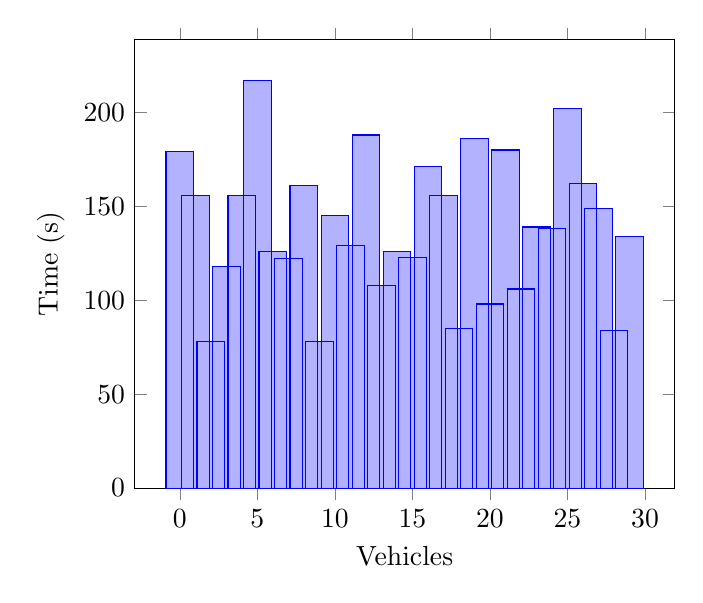
\begin{tikzpicture}
\begin{axis}[
legend style={anchor=west},
xlabel=Vehicles,
ylabel=Time (s),
ymin=0,
ybar,
]
\addplot coordinates {
(0, 179)
(1, 156)
(2, 78)
(3, 118)
(4, 156)
(5, 217)
(6, 126)
(7, 122)
(8, 161)
(9, 78)
(10, 145)
(11, 129)
(12, 188)
(13, 108)
(14, 126)
(15, 123)
(16, 171)
(17, 156)
(18, 85)
(19, 186)
(20, 98)
(21, 180)
(22, 106)
(23, 139)
(24, 138)
(25, 202)
(26, 162)
(27, 149)
(28, 84)
(29, 134)
};

\end{axis}
\end{tikzpicture}
\label{tik:100:19_O, 19_O.-60, 17_N, 15_S, 15_S.-30, 13_N, 13_N.-40, 11_N, 8_N, 7_N, 7_N.-60, 5_N, 4_N, 4_N.-60, 1_N}
\caption{100 percent diving with GSC on route $19_O, 19_O.-60, 17_N, 15_S, 15_S.-30, 13_N, 13_N.-40, 11_N, 8_N, 7_N, 7_N.-60, 5_N, 4_N, 4_N.-60, 1_N$}
\end{figure}
